\documentclass[tikz,border=8pt]{standalone}
\usepackage{amsmath}
\usetikzlibrary{arrows.meta,calc}
\definecolor{ink}{HTML}{17324D}
\definecolor{teal}{HTML}{168C80}
\definecolor{gold}{HTML}{D79A2B}
\definecolor{rose}{HTML}{C85B70}
\begin{document}
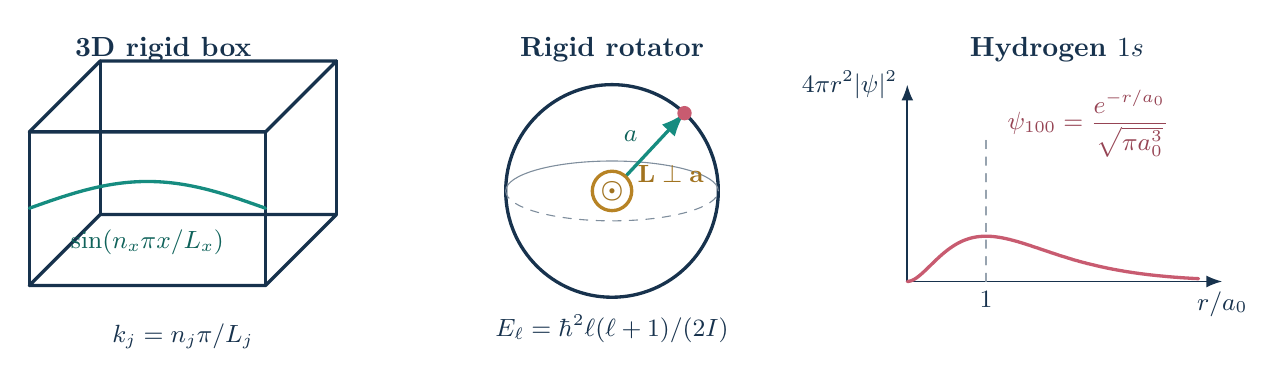
\begin{tikzpicture}[line cap=round,line join=round,>=Latex,font=\small]
  % Panel 1: rigid rectangular box.
  \begin{scope}[xshift=0cm]
    \node[font=\bfseries,text=ink] at (2.2,3.2) {3D rigid box};
    \coordinate (A) at (0.5,0.2);
    \coordinate (B) at (3.5,0.2);
    \coordinate (C) at (4.4,1.1);
    \coordinate (D) at (1.4,1.1);
    \coordinate (E) at (0.5,2.15);
    \coordinate (F) at (3.5,2.15);
    \coordinate (G) at (4.4,3.05);
    \coordinate (H) at (1.4,3.05);
    \draw[very thick,ink] (A)--(B)--(C)--(D)--cycle;
    \draw[very thick,ink] (E)--(F)--(G)--(H)--cycle;
    \draw[very thick,ink] (A)--(E) (B)--(F) (C)--(G) (D)--(H);
    \draw[very thick,teal,domain=0:3,samples=80,variable=\x]
      plot ({0.5+\x},{1.18+0.34*sin(180*\x/3)});
    \node[text=teal!70!black] at (2,0.75) {$\sin(n_x\pi x/L_x)$};
    \node[text=ink,align=center] at (2.45,-0.45)
      {$k_j=n_j\pi/L_j$};
  \end{scope}

  % Panel 2: rigid rotator on a sphere.
  \begin{scope}[xshift=6.0cm]
    \node[font=\bfseries,text=ink] at (1.9,3.2) {Rigid rotator};
    \coordinate (O) at (1.9,1.4);
    \draw[very thick,ink] (O) circle (1.35);
    \draw[dashed,ink!55] ($(O)+(-1.35,0)$) arc[start angle=180,end angle=360,x radius=1.35,y radius=.38];
    \draw[ink!55] ($(O)+(1.35,0)$) arc[start angle=0,end angle=180,x radius=1.35,y radius=.38];
    \coordinate (P) at ($(O)+(47:1.35)$);
    \draw[very thick,teal,-{Latex[length=3mm]}] (O)--(P) node[midway,above left,text=teal!70!black] {$a$};
    \fill[rose] (P) circle (2.6pt);
    \node[draw=gold!85!black,circle,very thick,inner sep=1.2pt,
      text=gold!75!black,fill=white] at (O) {$\boldsymbol{\odot}$};
    \node[anchor=west,text=gold!75!black] at ($(O)+(0.20,0.22)$)
      {$\mathbf L\perp\mathbf a$};
    \node[text=ink] at (1.9,-0.35) {$E_\ell=\hbar^2\ell(\ell+1)/(2I)$};
  \end{scope}

  % Panel 3: hydrogen radial probability generated from r^2 exp(-2r/a0).
  \begin{scope}[xshift=11.4cm]
    \node[font=\bfseries,text=ink] at (2.15,3.2) {Hydrogen $1s$};
    \draw[->,semithick,ink] (0.25,0.25)--(4.25,0.25) node[below] {$r/a_0$};
    \draw[->,semithick,ink] (0.25,0.25)--(0.25,2.75) node[left,align=center] {$4\pi r^2|\psi|^2$};
    \draw[very thick,rose,domain=0:3.7,samples=150,variable=\r]
      plot ({0.25+\r},{0.25+4.25*\r*\r*exp(-2*\r)});
    \draw[dashed,ink!45] (1.25,0.25)--(1.25,2.05);
    \node[below,text=ink] at (1.25,0.25) {$1$};
    \node[text=rose!75!black,align=center] at (2.55,2.25)
      {$\psi_{100}=\dfrac{e^{-r/a_0}}{\sqrt{\pi a_0^3}}$};
  \end{scope}
\end{tikzpicture}
\end{document}
